
% JuliaCon proceedings template
\documentclass{juliacon}
\setcounter{page}{1}


\usepackage{caption}
\usepackage{subcaption}
\usepackage{amsmath}
\usepackage{tikz}
\usepackage{pgfplots}
\pgfplotsset{compat=newest}
\usepackage{siunitx}
\usepackage{here}
\newcommand\todo[1]{\textcolor{red}{\textbf{TODO: #1}}}

%\usetikzlibrary{external}
%\tikzexternalize[prefix=figures/]

\begin{document}

% **************GENERATED FILE, DO NOT EDIT**************

\title{DeconvOptim.jl - Signal Deconvolution with Julia}

\author[1, 2]{Felix Wechsler}
\author[1, 2, 3]{Rainer Heintzmann}
\affil[1]{Faculty of Physics and Astronomy, Friedrich-Schiller-University,Jena, Germany}
\affil[2]{Leibniz Institute of Photonic Technology, Albert-Einstein-Straße 9,07745 Jena, Germany}
\affil[3]{Institute of Physical Chemistry and Abbe Center of Photonics, Friedrich-Schiller-University, Helmholtzweg 4, Jena, Germany}

\keywords{Julia, Image Processing, Deconvolution, Microscopy}

\hypersetup{
pdftitle = {DeconvOptim.jl - Image Deconvolution with Julia},
pdfsubject = {JuliaCon 2019 Proceedings},
pdfauthor = {Felix Wechsler, Rainer Heintzmann},
pdfkeywords = {Julia, Image Processing, Deconvolution, Microscopy},
}


\maketitle

\begin{abstract}
Deconvolution is a versatile method to enhance the quality of signals measured with systems which can 
be expressed mathematically as a convolution of a system's response function with a signal. 
In this paper, we present \verb|DeconvOptim.jl|, a flexible toolbox written in Julia to deconvolve one or multiple multi-dimensional signals which have been
degraded by a multi-dimensional signal response function. 
\verb|DeconvOptim.jl| works both on CPUs and GPUs and utilizes recent advancements in Julias automatic differentiation ecosystem. 

In this work we demonstrate that \verb|DeconvOptim.jl| surpasses the performance of existing open source libraries clearly
and is applicable to one dimensional time series datasets but also to multi-dimensional microscopical imaging datasets.
\end{abstract}


\section{Introduction}
Deconvolution has been a long addressed problem especially in astronomical imaging, digital signal processing or microscopy imaging.
The assumption is that images are degraded by some kind of blur which can be described as a convolution of a kernel $h$ with the image $S$:
\begin{equation}
    I(\mathbf r) = (h * S)(\mathbf r)
\end{equation}
where $*$ denotes a convolution operation.
$h$ is often called the point spread function (PSF) since it characterizes how the systems maps a point in the object to a blurred spot 
in the image.
Often this convolution operation is disturbed by different types of noise where the most common are additive Gaussian noise (e.g. due to the read out of the camera sensors) or Poisson shot noise (e.g. due to the quantum nature of photons):
\begin{align}
    Y_{\text{Poisson}}(\mathbf r) &= \text{Poisson}[(h * S)(\mathbf r)]\\
    Y_{\text{Gauss}}(\mathbf r) &= (h * S)(\mathbf r) + \text{Gauss}_{\sigma}(\mathbf r)
\end{align}
Due to noise and the low pass filter effect of the PSF, deconvolution is an ill-posed problem which cannot be solved directly.\\
A well known approach, because of its simplicity, has been the iterative Richardson-Lucy deconvolution algorithm 
\cite{Richardson:72}, \cite{lucy:74} for Poisson noise degraded signals.
Another common method is the non-iterative Wiener filter \cite{wiener2013extrapolation} because of its predictable runtime.
The Wiener filter assumes additive noise which is often not a good approximation, especially in low light conditions as in microscopy or astronomy. 
Recently, machine learning based methods have become more and more favoured in deconvolution because
of the possibility to add learned properties of similar images to the algorithm \cite{Kruse_2017_ICCV}.
However, those implementations are usually restricted to cases where experimental datasets are available for the characterization and training.
\verb|DeconvOptim.jl| is a toolbox written in Julia \cite{bezanson2017julia} which offers several deconvolution algorithms 
like the iterative Richardson-Lucy algorithm but also
much more flexible methods which are based on minimizing a 
noise-dependent loss function with the help of modern gradient-descent minimization routines. 
Also this toolbox is not restricted in dimensionality and therefore can be applied to deconvolution problems in many different fields.

\section{Efficient Convolutions}
The mathematical definition of a convolution is
\begin{equation}
    (h * S)(\mathbf r) = \int_{-\infty}^{\infty} h(\mathbf r - \mathbf x) \cdot S(\mathbf x) \, \mathrm d \mathbf x.
    \label{eq:conv}
\end{equation}
To obtain efficient deconvolution algorithms we also need an efficient way to calculate the convolution operations.
Today, convolution operations of spatially small kernels $h$ can be calculated on GPUs very efficiently in real space.
However, often the blurring kernel $h$ is not spatially small and might be also multi-dimensional. In that case, FFT based convolutions
outperform sliding kernels. In microscopy and astronomy that is often the case, since a defocus broadens the PSF.

\subsection{FFT Based Convolution}
    The basis for fast convolution calculation via Fourier transforms lies in the convolution theorem. It states that
    \begin{equation}
        \mathcal F\left\{(h * S)\right\}(\mathbf k) = \mathcal F\{h\} (\mathbf k) \cdot \mathcal F\{S\} (\mathbf k),
        \label{eq:fftconv}
    \end{equation} 
        which means that a Fourier transform $\mathcal F$ of a convolution operation is equivalent to a point wise multiplication of the Fourier transforms 
        of $h$ and $S$.
        Fortunately, the Fourier transform operations can be calculated even for moderate large 3D arrays quickly on modern computing machines via
        the Fast Fourier Transform (FFT).
        In Julia, \verb|FFTW.jl| offers a convenient interface to the FFTW library \cite{FFTW05}.
        The time complexity to calculate \autoref{eq:fftconv} is $\mathcal{O}(N \cdot \log N)$ for a one dimensional discretized dataset with $N$ samples.
        For a 2D dataset with size $N \times M$ it is $\mathcal{O}(N \cdot M \log(N \cdot M))$ and accordingly for higher dimensions.
        Spatially based convolution kernels with size $K \times L$ applied on an image with
        $N \times M$ data points have a runtime of $\mathcal O(N \cdot M \cdot K \cdot L)$.
        It is clear that for larger kernel sizes ($K,L \gg 1$) the sliding method 
        has worse computational complexity than the FFT based convolutions. The many cores of a GPU can mitigate that to a certain extent
        but since the FFT (CuFFT in the CUDA library \cite{CUDA}) can be also executed in parallel fashion, 
        both approaches profit from parallelization.
        

\subsection{Wrap-Around Artifacts in FFT based Convolutions}
    One drawback of a FFT based convolution are wrap-around artifacts (see arrow in \autoref{fig:withoutpad}). The reason is, that the FFT operation calculates the discrete
    Fourier transform (DFT) which inherently assumes periodic data. If one applies a FFT on a finite data set the assumption is that
    this finite data set repeats itself. 
    To weaken the wrap-around artifacts in the convolution one can zero or mean pad the image before convolution 
    and remove the padding afterwards. Such approaches still suffer from artifacts when boundary values do not fit
    to the mean or to zero as it can be observed in \autoref{fig:withpad} where the arrow is pointing to.
    \begin{figure}[h]
        \centering
        \begin{subfigure}[b]{.25\textwidth}
            \centering
            \begin{tikzpicture}[scale=0.7]
                \node at (0,0) {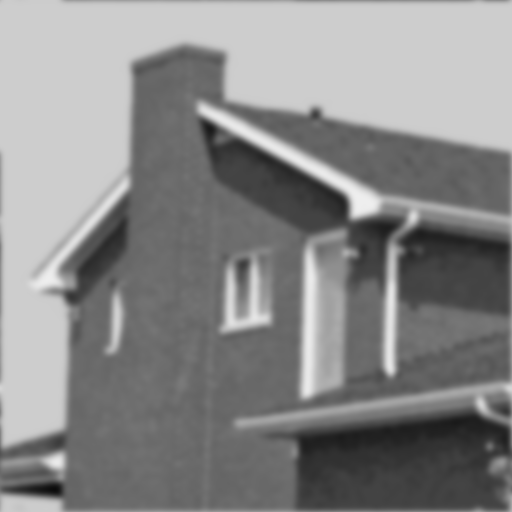
\includegraphics[width=.63\textwidth]{figures/full_house_no_pad.png}};
                \draw[red] (-2.0, -1.6) rectangle (-1.6, -1.2);
                \node[color=red] at (0,0) {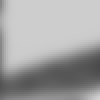
\includegraphics[width=.28\textwidth]{figures/edge_house_no_pad.png}};
                \draw[color=red] (-0.91, -0.9) rectangle (0.9, 0.9); 
                \draw[color=red] (-2.0, -1.2) -- (-0.9, 0.9);
                \draw[color=red] (-1.6, -1.6) -- (0.9, -0.9);
                \draw[<-, color=red, thick ](-0.85, 0) -- (-0.4, 0.6);
            \end{tikzpicture}
            \caption{Without padding}
            \label{fig:withoutpad}
        \end{subfigure}%
        \begin{subfigure}[b]{.25\textwidth}
            \centering
            \begin{tikzpicture}[scale=0.7]
                \node at (0,0) {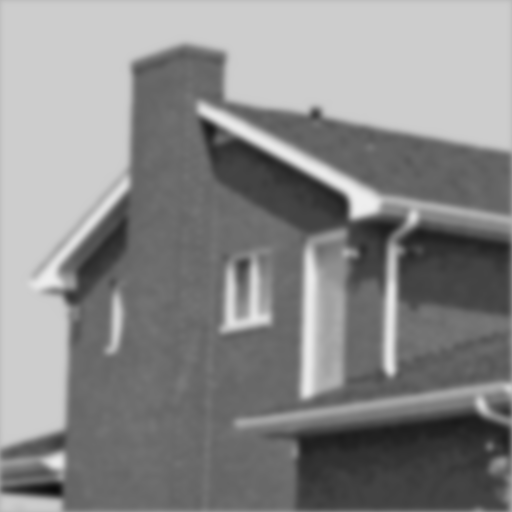
\includegraphics[width=.63\textwidth]{figures/full_house_pad.png}};
                \draw[red] (-2.0, -1.6) rectangle (-1.6, -1.2);
                \node[color=red] at (0,0) {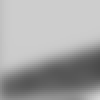
\includegraphics[width=.28\textwidth]{figures/edge_house_pad.png}};
                \draw[color=red] (-0.90, -0.9) rectangle (0.9, 0.9); 
                \draw[color=red] (-2.0, -1.2) -- (-0.9, 0.9);
                \draw[color=red] (-1.6, -1.6) -- (0.9, -0.9);
                \draw[<-, color=red, thick ](-0.8, -0.7) -- (-0.3, -0.3);
            \end{tikzpicture}
            \caption{With padding.}
            \label{fig:withpad}
        \end{subfigure}
        \caption{Comparison between two blurred images. The image a) is a straightforward FFT based blurred image.
        The zoomed region shows dark artifacts at the left side originated from the right hand side. Also at the top of the image some dark regions from
        the bottom scattered into the bright sky.
        Image b) was padded before blurring with 10 pixels on each side with value 0.7 which results in bright regions around the image. The blur kernel was a Gaussian kernel
        with standard deviation $\sigma=\SI{3}{pixel}$.}
        \label{fig:}
    \end{figure}
    To solve for the wrap-around artifacts in deconvolution we use a different approach which will be presented in \autoref{sec:wrap}. 
\subsection{Preferred Convolution}
The current state of \verb|DeconvOptim.jl| uses the FFT approach to calculate the convolution.
However, in principle one could add the possibility to choose spatially based convolutions.
But since the runtime gets especially long in multi-dimensional signal deconvolution where FFT based methods
are faster, we always use FFT based convolutions here. 
   
\section{Inverse Modelling}
In \autoref{fig:pipeline} we show our approach to deconvolution.
The general idea is to create a (physical) forward model describing the measurement process.
\begin{figure}[h]
    \centering
    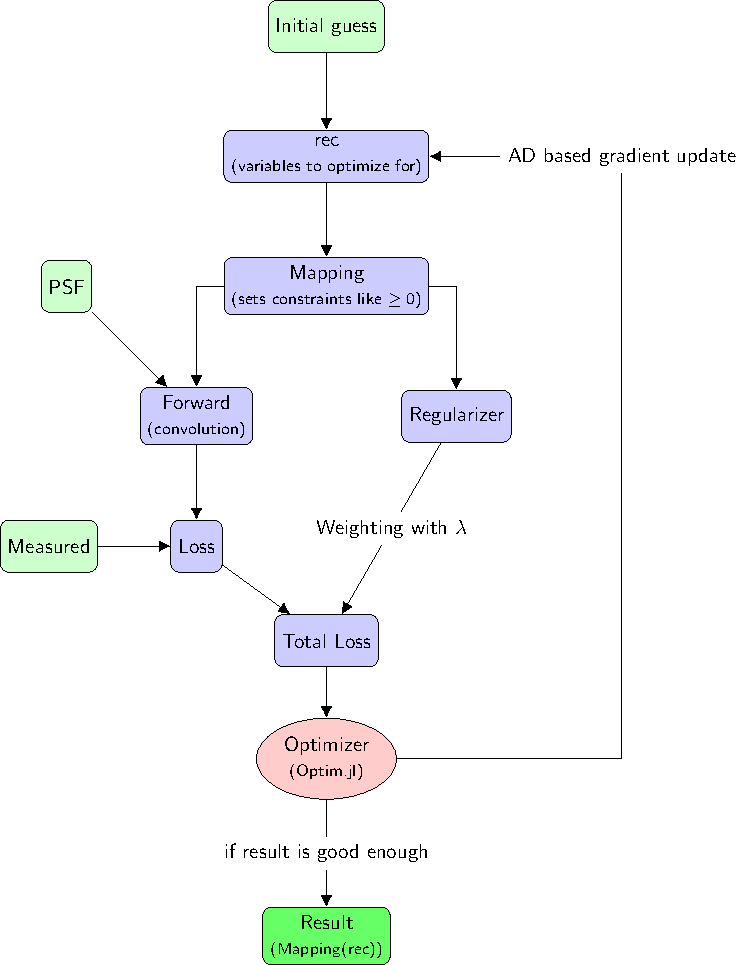
\includegraphics[width = .4\textwidth]{figures/pipeline.pdf}
    \caption{General pipeline of our deconvolution approach.}
    \label{fig:pipeline}
\end{figure}

At the beginning of the optimization we start with an initial guess $x(\mathbf r)$. 
Via a mapping function we can impose some restrictions to the final solution (e.g. non-negativity, value intervals).
The forward model is then applied to the mapped reconstruction. We provide a default function where 
the forward function is a convolution but we also allow to plug in a different forward model.
This output of the forward function is compared
to our noisy measurement under a given loss function.
Since deconvolution is an ill-posed problem, we regularize the loss function with a regularizer.
Afterwards we calculate the gradient of the loss function with respect to the reconstruction $x(\mathbf r)$ via automatic differentiation (AD).
The values of the total loss and the gradient are then used by an optimizer (to minimize the total loss) to apply a gradient descent optimization to get a proper reconstruction.\\

As typical for Julia packages, except \verb|FFTW.jl| and \verb|CUDA.jl| \cite{besard2018juliagpu}, all code is written in Julia.
Therefore it is easy to replace the forward model with any Julia code, as long as we can 
automatically differentiate through the code. The gradient step is currently calculated with the reverse mode AD of \verb|Zygote.jl| \cite{Zygote.jl-2018}. 
As default for the optimization we use the L-BFGS \cite{LBFGS} routine provided by \verb|Optim.jl| \cite{mogensen2018optim}.
L-BFGS is suitable for optimization with many million parameters as it only stores a sparse representation of the inverse Hessian matrix,
which is built from a finite number of past function and gradient evaluations. 
Results are often good after 10 to 50 iterations whereas Richardson-Lucy takes
a few hundreds iterations. 
However, as we will see later due to the more complex optimization routine the speed-up in using L-BFGS is for a simple 
deconvolution minor.



\subsection{Mapping Function}
    Mapping functions are an easy way to constrain the resulting reconstruction to predefined ranges.
    For example, if the optimizer optimizes the variables $\text{rec}$ which are then squared, we know that
    $\text{rec}^2$ is definitely non-negative. Instead of directly using $\text{fwd}(\text{rec})$ we compare
    $\text{fwd}(\text{rec}^2)$ with the measurement $Y$ where $\text{fwd}$ is the function describing the physical operation (mostly 
            a convolution). 
    This mapping function does not change the outcome as long
    as it is an surjective function for the desired number space (e.g. a parabola is non-negative and covers all positive values) 
    and does not change the convexity of a problem.
    Functions like shifted $\tanh$ are possible as well since it is an bijective function in $[-1, 1]$ and monotonic increasing
    in the whole definition space.
    Hence the final result is $\text{rec}^2$ in case of the quadratic mapping.

\subsection{Wrap-around Artifacts Suppression}
    \label{sec:wrap}
    To prevent that wrap-around artifacts occur during deconvolution we can instead
    of reconstructing an object having the same size as the measurement, reconstruct
    an object having a slightly larger size. This is shown in \autoref{fig:wrap_around}.
    \begin{figure}[h]
        \centering
        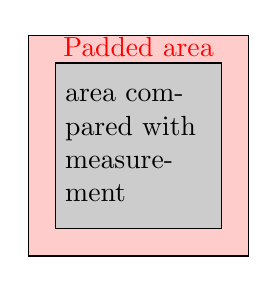
\begin{tikzpicture}[scale=0.7]
            \draw[fill=red!20!white] (0,0) rectangle (4,4);
            \node[color=red] at (2, 3.8) {Padded area};
            \draw[fill=gray!40!white] (0.5,0.5) rectangle (3.5,3.5); 
            \node[text width=2.0cm, color=black] at (2.1, 2) {area compared with measurement};
        \end{tikzpicture}
        \caption{Reconstructed data is padded before deconvolution but only the red region is compared with the measurement.}
        \label{fig:wrap_around}
    \end{figure}
    Consequently, we only compare the grey part of the reconstruction with the measurement.
    Through the AD and the convolution operations we still optimize for the whole area (including the red one).
    With that padding we reduce that images on the boundary influence in circular manner on reconstruction in the grey area.


\section{Loss Function}
    Apart from forward model, the loss function is the most critical part in the optimization.
    It has to account for the noise created by the measurement process or instrument. 

\subsection{Poisson Data Term}
    Poisson shot noise is often the dominant source of noise hence we 
    explain the details.
    The key is to interpret the measurement as a stochastic process. 
    Our aim is to find a deconvolved image which predicts the measured image as accurately as 
    possible.
    Mathematically the probability for a certain measurement $Y$ under Poisson noise is


\begin{equation}
    p(Y(\mathbf r)|\mu(\mathbf r)) = \prod_r \frac{\mu(\mathbf r)^{Y(\mathbf r)}}{\Gamma(Y(\mathbf r) + 1)} \exp(- \mu(\mathbf r))
\end{equation}

where $Y$ is the measurement, $\mu$ is the expected measurement (ideal measurement without noise) and $\Gamma$ is the generalized factorial function.
In the deconvolution process we get $Y$ as measured input and want to find the ideal specimen $S$ which results in a measurement $\mu(\mathbf r) = (S * \text{PSF})(\mathbf r)$.
Since we want to obtain the best reconstruction, we want 
to find a $\mu(\mathbf r)$ so that $p(Y(\mathbf r) | \mu(\mathbf r))$ gets maximized.
Because that means
that we find the specimen which describes the measurement with the highest probability.
Instead of maximizing $p(Y(\mathbf r) | \mu(\mathbf r))$ a common trick is to minimize $- \log(p(Y(\mathbf r)|\mu(\mathbf r)))$. 
Mathematically, the optimization of both functions provides same results but the latter is numerically more stable.

\begin{align}
&\underset{S(\mathbf r)}{\arg \min} (- \log(p(Y(\mathbf r)|\mu(\mathbf r)))) =\\ &\underset{S(\mathbf r)}{\arg \min} \sum_r \mu(\mathbf r) + \log(\Gamma(Y(\mathbf r) + 1)) - Y(\mathbf r) \log(\mu(\mathbf r))
\end{align}

which is equivalent to

\begin{equation}
    \underset{S(\mathbf r)}{\arg \min}\, L = \underset{S(\mathbf r)}{\arg \min} \sum_r (\mu(\mathbf r)  - Y(\mathbf r) \log(\mu(\mathbf r))
    \label{eq:poisson_loss}
\end{equation}

since the second term only depends on the constant $Y(\mathbf r)$ but not on $\mu(\mathbf r)$.
The gradient of $L$ with respect to $\mu(\mathbf r)$ is simply

\begin{equation}
    \nabla L = 1 - \frac{Y(\mathbf r)}{\mu(\mathbf r)}
    \label{eq:gradpoisson}
\end{equation}

The function $L$ and the gradient $\nabla L$ are needed for any gradient descent optimization algorithm.
The numerical evaluation of the Poisson loss can lead to issues. Since $\mu(r)=0$ can happen for a measurement with zero intensity background. However, the loss is not defined for $\mu \leq 0$. In our source code we set all intensity values below a predefined threshold $\epsilon$ to $\epsilon$ itself. This prevents the evaluation of the logarithm at undefined values.
The final source code has a modified version of \autoref{eq:gradpoisson} as registered gradient for \autoref{eq:poisson_loss}.
The reason is, that for values of $\mu(\mathbf r) = 0$ the equation is not defined and has to be handled separately. 

\subsection{Regularizer}
    The regularizer is an additional part in the total loss to add some additional priors like sparsity and smoothness.
    Most real samples are smooth over large regions and such regularizers enhance the quality of the reconstruction.
    In our toolbox we currently implement several regularizer like (smoothed) Total variation, Good's roughness \cite{Verveer:98}, \cite{Good:71} and Tikhonov. 
    \subsubsection{Total Variation as example}
        As the name suggests, Total variation tries to penalize variation in the image intensity. Therefore it sums up the gradient strength at each point
        of the image:
        \begin{equation}
            \text{Reg}(S(\mathbf r)) = \sum_r  |(\nabla S)(\mathbf r)|
        \end{equation}
        Since we look at the magnitude of the gradient strength, this regularizer is anisotropic.
        In 2D TV is defined like: 
        \begin{equation}
        \begin{split}
            \text{Reg}(S(\mathbf r)) = \sum_{x,y} \big[& |S(x + 1, y) - S(x, y)|^2 \\[-0.4cm] 
                                                & + |S(x, y + 1) - S(x, y)|^2\big]^{\frac12}
        \end{split}
        \end{equation}
        In many frameworks such a regularizer is implemented via functions like \lstinline{circshift}. 
        However, such approaches create often several copies of the data. 
        We currently use \verb|Tullio.jl|\cite{michael_abbott_2021_5047410} to create efficient functions 
        calculating the regularizer and the gradient. For simple expressions
        such as below, \verb|Tullio.jl| registers an analytical gradient and therefore allows to apply the same efficient mechanisms 
        to the gradient calculation which have been used for the regularizer evaluation itself.
        A (smoothed) Total variation with \verb|Tullio.jl| is defined here:
        \begin{lstlisting}[language = Julia]
function total_variation(arr, ϵ=eltype(arr)(1e-8))
    @tullio r = sqrt(ϵ + 
                abs2(arr[i,j] - arr[i+1,j]) +
                abs2(arr[i,j] - arr[i,j+1]))
end
        \end{lstlisting}
        \lstinline{ϵ} is needed for regions where \lstinline{arr == 0} because otherwise the gradient returns infinite values.
        Note, that definition just demonstrates how the regularizer can be written down.
        In our toolbox we allow for much more options. Since \verb|Tullio.jl| cannot handle generic multi-dimensional data yet
        we create regularizers which can vary in step size, dimensionality and
        different weighting in dimensions via Julia's metaprogramming capability.
        A call like 
        \begin{lstlisting}[language = Julia]
julia> using DeconvOptim

julia> reg = TV(num_dims=4, sum_dims=[1,2,3],
                weights=[1,1,2])
#169 (generic function with 1 method)

julia> reg(randn((10,20,30,40)))
417810.11332404887
        \end{lstlisting}
        results in a regularizer accepting four dimensional arrays. However, the regularization only happens along the first three dimension
        and the third dimensions is weighted differently.
        Such options are available for most of the regularizers implemented in our toolbox.

\section{Experiments}
    In this section we show some experiments and compare parts of the software to other solutions.
All experiments were executed on Ubuntu 20.04 using a AMD Ryzen 5 5600X 6-Core processor (12 threads) with \SI{32}{GB} DDR4 RAM and Julia 1.6.2.
    If possible, all threads were used.
    As GPU accelerator we used a GeForce RTX 2060 SUPER with \SI{8}{GB} memory and CUDA 11.3 and CUDA.jl 3.3.1.
    Our experiments additionally made use of the following packages in Julia 1.6.2: ArrayInterface.jl\cite{DifferentialEquations.jl-2017}, 
    BenchmarkTools.jl\cite{BenchmarkTools.jl-2016}, FFTW.jl\cite{FFTW05}, LLVM.jl\cite{LLVM.jl-2017}, Optim.jl\cite{mogensen2018optim}
    and  Zygote.jl\cite{Zygote.jl-2018}. 
    \subsection{One-Dimensional Time Series}
        First, we want to demonstrate the deconvolution of an artificial one dimensional dataset blurred with a certain PSF.
        Additionally, we want to demonstrate the mechanism to reduce wrap-around artifacts in the deconvolution.
        On the left hand side in \autoref{fig:1D_dataset} we can see a data series which has been simulated 
        as a convolution with a PSF and degradation with additive Gaussian noise.
        \begin{figure}[H]
            \begin{subfigure}[b]{.25\textwidth}
                \centering
                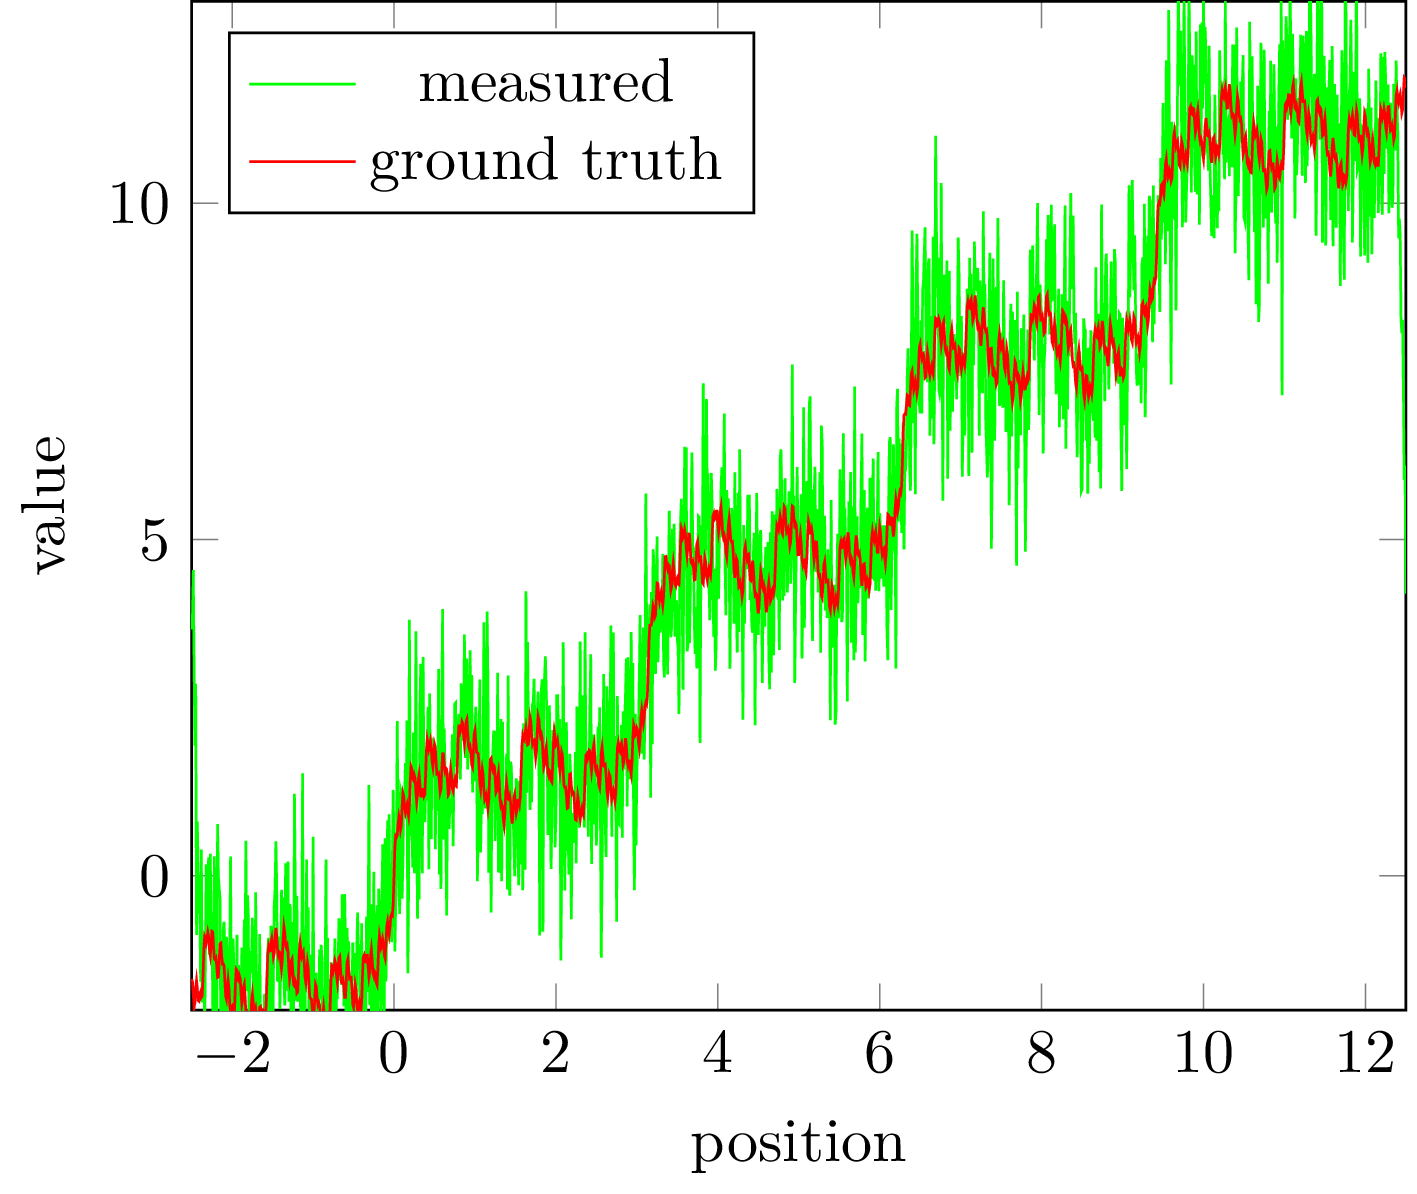
\includegraphics[width=\textwidth]{figures/1d_plot_data_blurred.png}
                \caption{}
                \label{fig:1D_dataseta}
            \end{subfigure}%
            \begin{subfigure}[b]{.25\textwidth}
                \centering
                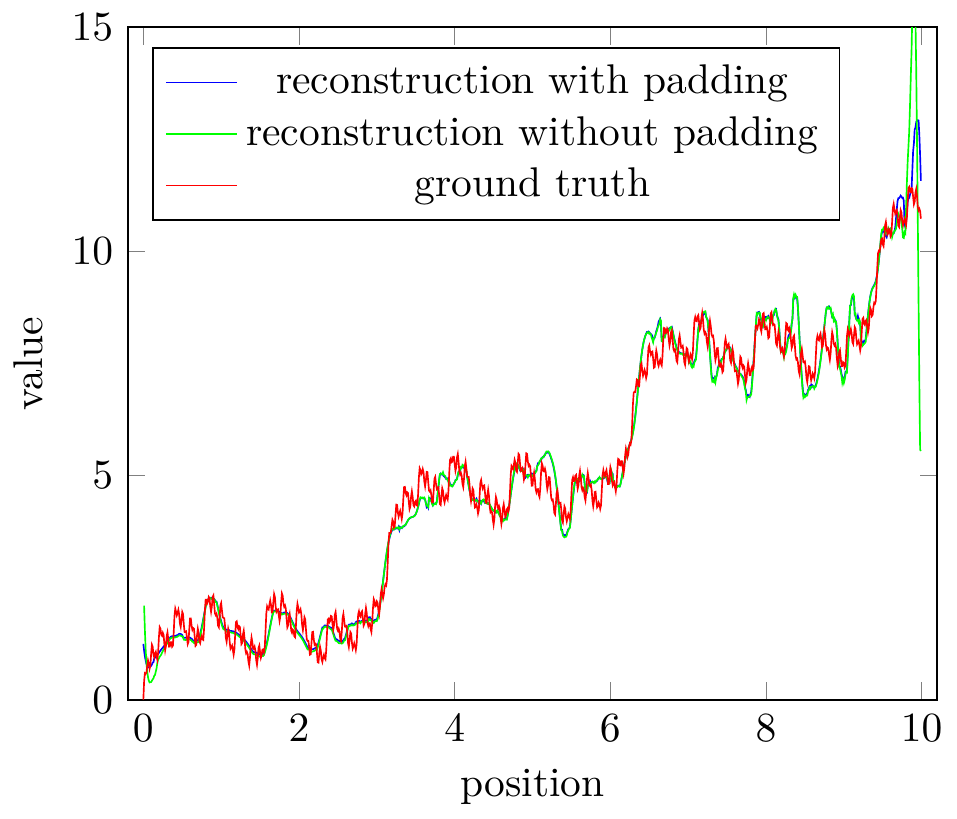
\includegraphics[width=\textwidth]{figures/1d_plot_data_res_pad_vs_nopad.png}
                \caption{}
                \label{fig:1D_datasetb}
            \end{subfigure}
            \caption{1D data which has been convolved with a PSF and was degraded with additive Gaussian noise with $\sigma=1.0$. Note that for the deconvolution we have chosen a position interval which is well within the full series so that there are not wrap-around artifacts in the measurement.}
            \label{fig:1D_dataset}
        \end{figure}
        On the right hand we can see the results of the following deconvolution.
    The first statement applies a total padding of $1$ meaning that the size is doubled and therefore the measured data is padded.
    As we can see, the blue curve in \autoref{fig:1D_datasetb} does not show these intense spikes at the boundaries as the green curve shows.
        \begin{lstlisting}[language=Julia]
r_p, o = deconvolution(measured, psf, loss=Gauss(),
     iterations=12, regularizer=TV(num_dims=1),
     λ=0.05, padding=1)
r, o = deconvolution(measured, psf, loss=Gauss(), 
     iterations=12, regularizer=TV(num_dims=1),
     λ=0.05, padding=0)
        \end{lstlisting}
    Also we notice that the deconvolved data in \autoref{fig:1D_datasetb} does not show all the details which are visible in the ground truth.
    The reason is that the PSF is a low pass filter and therefore only frequencies which have been passed through the filter 
    can be enhanced in terms of contrast in a deconvolved result.

    \subsection{Influence of Regularizer}
        In this part we want to demonstrate the influence of the regularizer.
        \autoref{fig:fabioa} is a simulated imaged which has been affected by Poisson shot noise and blurring by a PSF.
        \begin{figure}[h]
            \begin{subfigure}[b]{.16\textwidth}
                \centering
                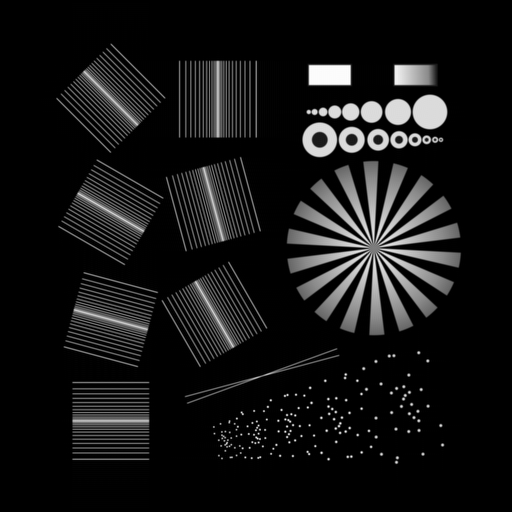
\includegraphics[width=0.99\textwidth]{figures/resolution_test_512.png}
                %\caption{Ground truth.}
                \caption{}
                \label{fig:gt}
            \end{subfigure}%
            \begin{subfigure}[b]{.16\textwidth}
                \centering
                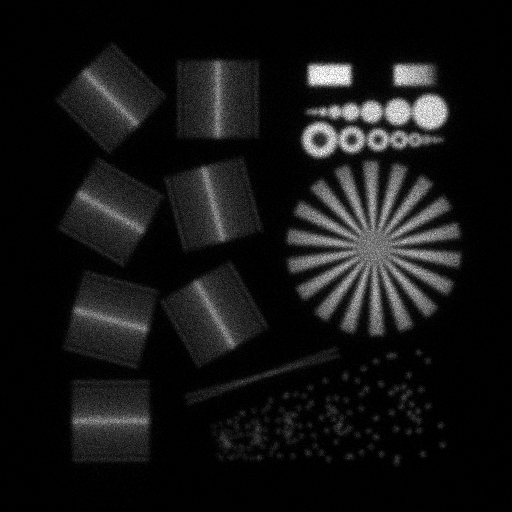
\includegraphics[width=.99\textwidth]{figures/resolution_test_chart_blurry.png}
                %\caption{Measured with Poisson noise}
                \caption{}
                \label{fig:fabioa}
            \end{subfigure}%
            \begin{subfigure}[b]{.16\textwidth}
                \centering
                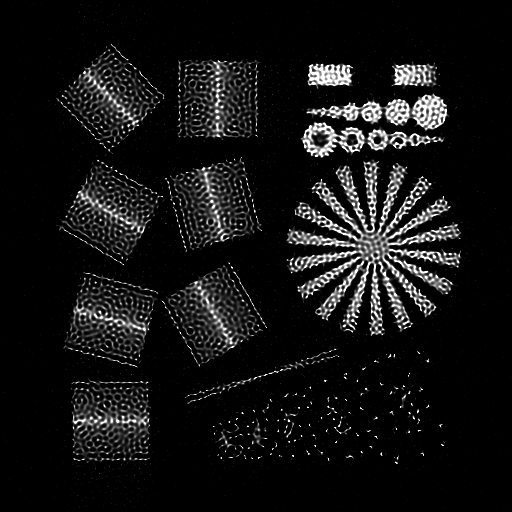
\includegraphics[width=.99\textwidth]{figures/resolution_test_chart_no_reg_iter_50.png}
                %\caption{Without regularizer $N=50$}
                \caption{}
                \label{fig:fabiob}
            \end{subfigure}%
            \hfill
            \begin{subfigure}[b]{.16\textwidth}
                \centering
                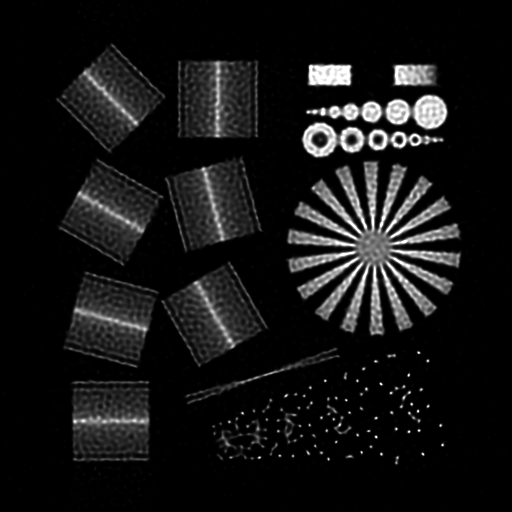
\includegraphics[width=0.99\textwidth]{figures/resolution_test_chart_no_reg_iter_10.png}
                %\caption{Without regularizer $N=10$}
                \caption{}
                \label{fig:fabioc}
            \end{subfigure}%            
            \begin{subfigure}[b]{.16\textwidth}
                \centering
                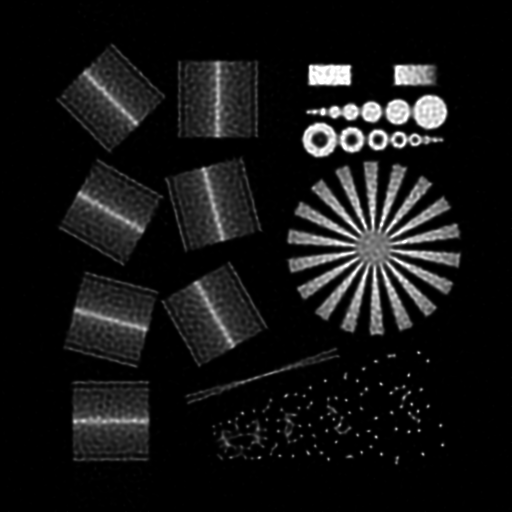
\includegraphics[width=0.99\textwidth]{figures/resolution_test_chart_regularizer_008_iter_21.png}
                %\caption{With regularizer $N=24$.}
                \caption{}
                \label{fig:fabiod}
            \end{subfigure}%            
            \caption{a) is the ground truth image. b) has been convolved with a PSF and affected by Poisson shot noise (100 photons expected for the brightest pixel). 
            c) is deconvolved for 50 iterations without a regularizer, d) for 10 iterations without a regularizer. e) converged with Good's roughness regularizer and 
                            after 24 iterations with $\lambda=0.03$.}
            \label{fig:image}
        \end{figure}

        This test chart is suited to judge the resolution of a reconstruction since the pieces of the Siemens star
        have decreasing spacing towards its middle which is equivalent to higher spatial frequencies.
        \autoref{fig:fabiob} shows the result after 50 iterations of the deconvolution. 
        We see that the image is heavily affected by some artifacts (the dotted patterns) which usually occur after too many iterations without a regularizer.
        Additionally, we notice that the core in the Siemens star is denser 
        requiring higher spatial resolution to resolve. 
        \autoref{fig:fabioc} shows the results after 10 iterations of the deconvolution without a regularizer.
        We have chosen 10 iterations since the normal cross correlation (NCC) shows the maximum at 10 iterations.
        Optimizing for more iterations seems to introduce more and more artifacts to the image as it can be seen visually as well.
        \autoref{fig:fabiod} shows the results after 24 iterations of the deconvolution but regularized with a Good's roughness regularizer.
        The total image quality is much better since the regularizer dampens the artifacts but also results in lower
        resolution. With the regularizer weight $\lambda$ one can adjust the regularization strength.
        In \autoref{fig:rel_energy_regain} we show the relative energy regain $G_\textrm{R}$ (REG) \cite{rel_energy_regain}.
        The meaning of the REG is how well certain frequencies are reconstructed in comparison
        to the ground truth. $G_\textrm{R} = 1$ is a perfect reconstruction, $G_\textrm{R} = 0$ indicates that 
        this frequency could not be recovered at all, $G_\textrm{R} < 0$ means that the reconstruction introduces 
        wrong information at this frequencies
        which are further from the ground truth than not reconstructing these frequencies. 
        \begin{figure}[h]
            \centering
            \begin{subfigure}[b]{.23\textwidth}
                \centering
                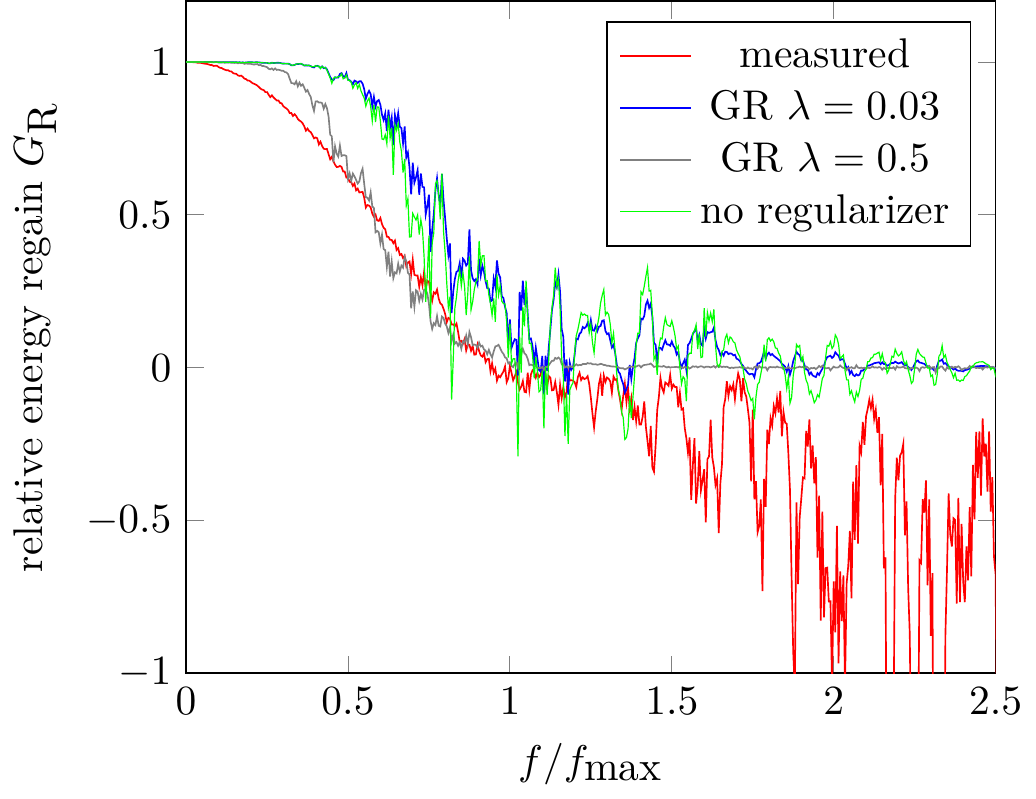
\includegraphics[width =\textwidth]{figures/test_chart_relative_energy_regain.png}
                \caption{REG $G_\textrm{R}$ over different frequencies.}
                \label{fig:rel_energy_regain}
            \end{subfigure}
            \hfill
            \begin{subfigure}[b]{.23\textwidth}
                \centering
                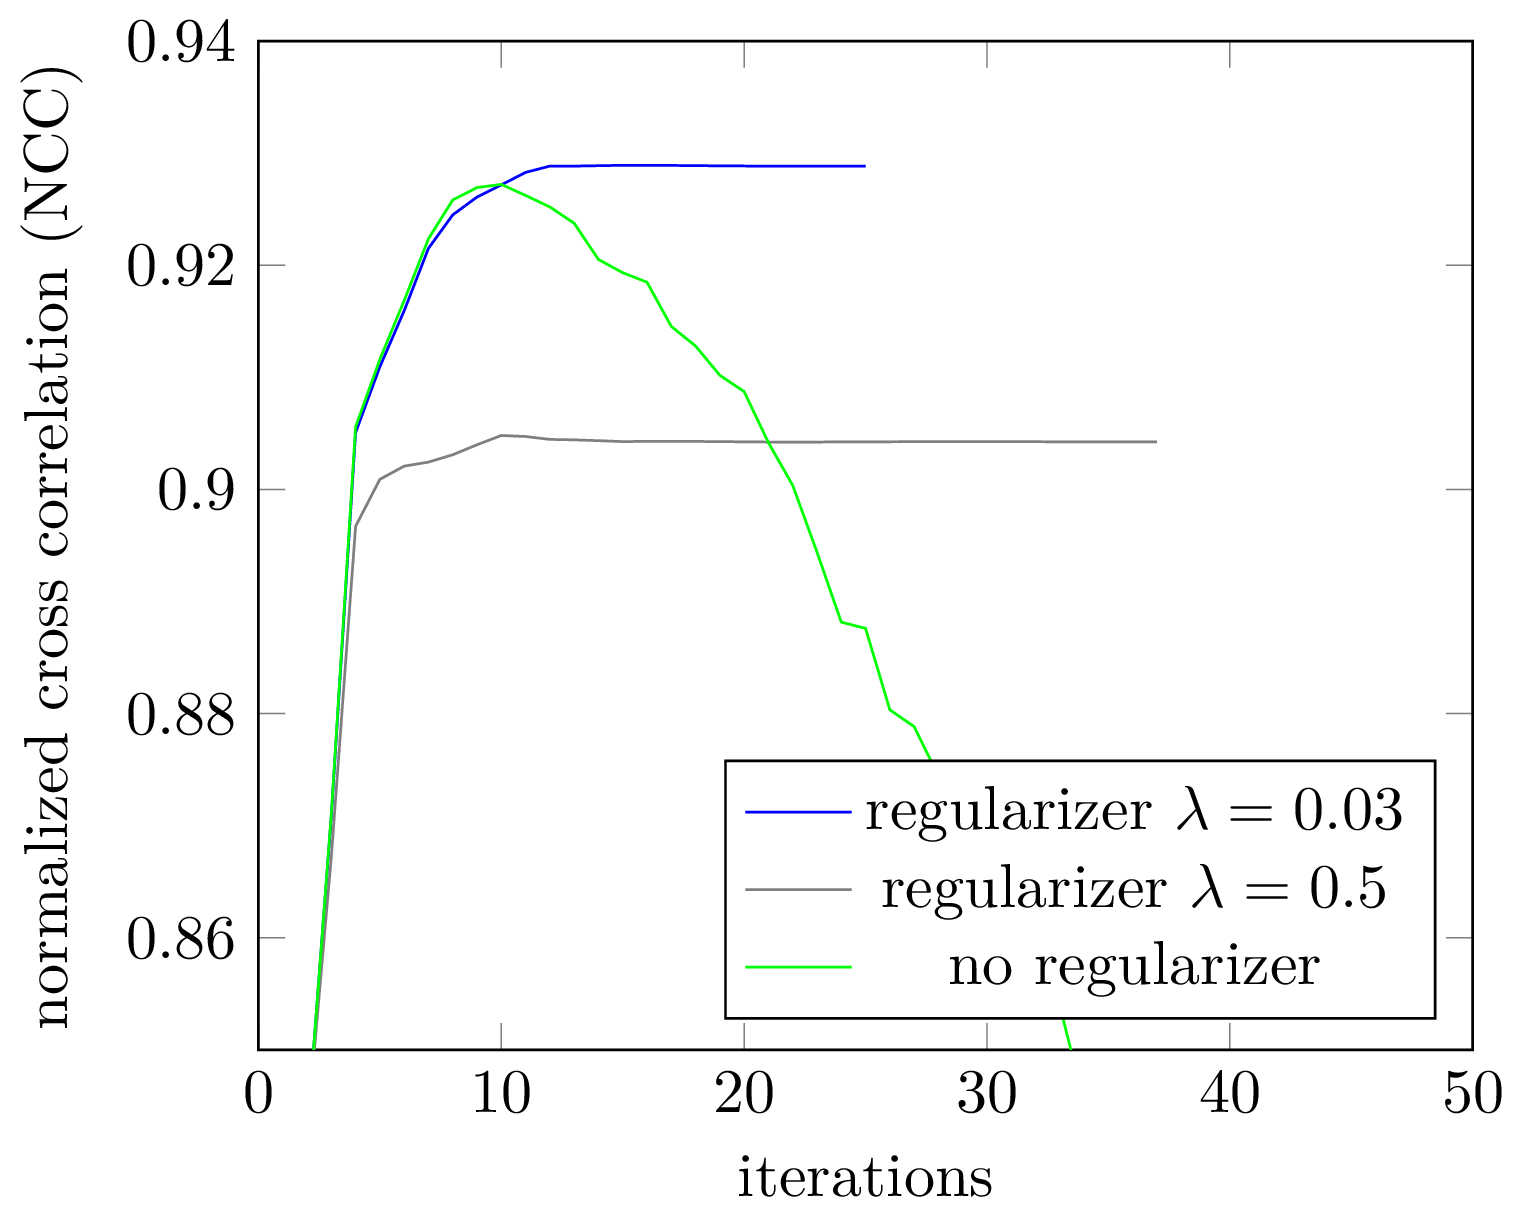
\includegraphics[width =1 \textwidth]{figures/test_chart_ncc.png}
                \caption{NCC over the number of iterations.}
                \label{fig:ncc}
            \end{subfigure}
            \caption{NCC and REG are quantitative measurements to judge the quality of a deconvolution result. 
                In a) we show the REG for the hand-optimized non-regularized version with 10 iterations and the (converged) regularized versions with $\lambda=0.03$ and $\lambda=0.5$.}
        \end{figure}
        We can see that the red measured curve shows the typical contrast loss until the maximum frequency $f_\textrm{max}$ (the PSF has
            zero transmittance over this frequency threshold).
        Beyond $f_\textrm{max}$ Poisson noise introduces fake frequencies.
        The green curve shows the REG of the deconvolution without a regularizer. 
        For regions below  $f_\textrm{max}$
        the deconvolution enhances the contrast. However, around and beyond $f_\textrm{max}$ several artifacts are introduced.
        The regularized blue curve performs better and only some frequencies show a REG below zero.
        To some extent the regularized version can also recover information above $f_\textrm{max}$ which are not supported by the PSF.
        \autoref{fig:ncc} shows the NCC over the number of iterations.
        Especially the deconvolution without a regularizer suffers from poor performance after a high number of iterations.
        Either one has to stop early after a hand optimized iteration number (here 10) or use a regularizer.
        The regularized version seems to be robust against a higher number of iterations and even converges after 24.
        In conclusion we can say that both the regularized and the non-regularized versions produce good results. 
        In the non-regularized one has to hand-optimize the number of iterations whereas in the regularized one has to optimize $\lambda$.
        However, without the ground truth image it is not clear which iteration or $\lambda$ is optimal and hence
        this depends on the user.
        Advantage of the non-regularized version is, that it performs more than twice as fast but as it can be seen in \autoref{fig:fabioc} 
        it shows slightly more artifacts in homogenous regions.

    \subsection{Multi-Dimensional Microscopy Data}
        To more completely demonstrate the features available in \verb|DeconvOptim.jl|,
        we deconvolve a four dimensional (three spatial dimensions and a color dimension) dataset where the measured volume consists of a 3D datasets
        with three different color channels, shown in \autoref{fig:result_3d}.
        Here we assumed a common single 3D PSF for all color channels.
        Julia's broadcast mechanism is able to understand that 
        the data has more dimensions that the PSF and expands the PSF so that a multiplication still works.
        \begin{figure}[h]
            \begin{subfigure}{.25\textwidth}
                \centering
                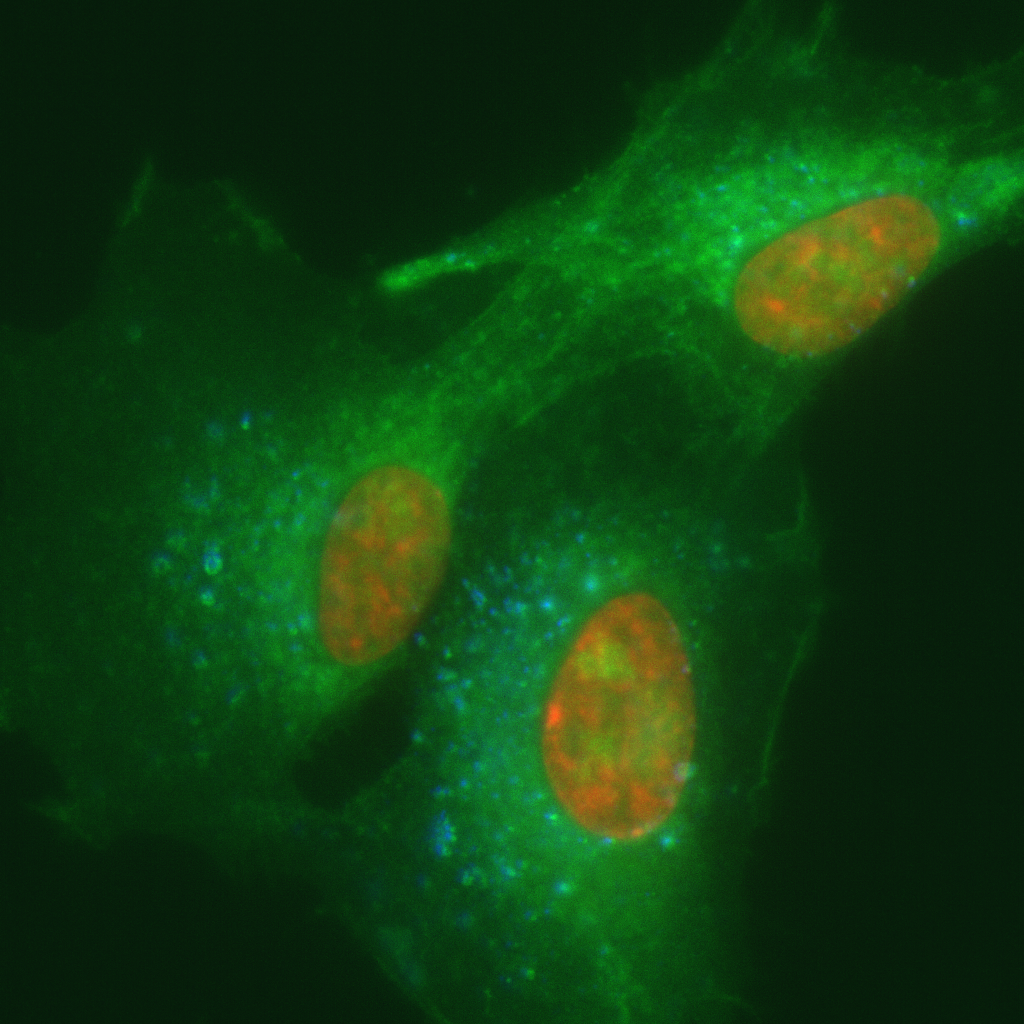
\includegraphics[width = .85\textwidth]{figures/raw_rgb.png}
            \end{subfigure}%
            \begin{subfigure}{.25\textwidth}
                \centering
                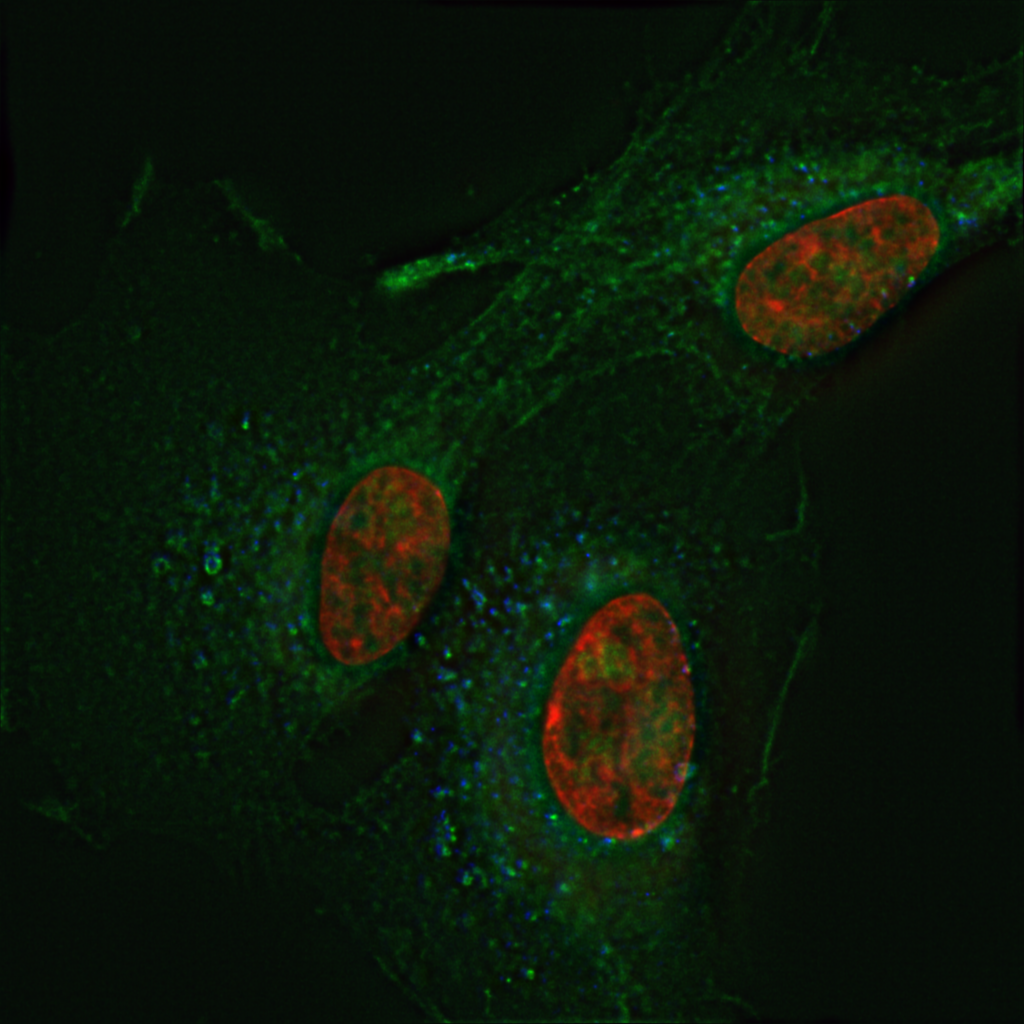
\includegraphics[width = .85\textwidth]{figures/deconvolved_rgb.png}
            \end{subfigure}
            \caption{Slice of a 3D dataset with three different colors. a) is the raw data and b) is the
                    deconvolved image.}
            \label{fig:result_3d}
        \end{figure} 
        We only need to specify for the FFT over which dimensions the convolution should happen.
        Clearly we can see that the deconvolution removed a lot of the background blur.

    \subsection{Performance Comparison}
        Since Julia is often advertised with great performance we compare parts and the full deconvolution to other implementations in
        terms of their total performance.
        \subsubsection{Regularizer}
            In \autoref{tab:reg} we can see the runtimes for different TV regularizer implementations. As we can see, \verb|Tullio.jl| outperforms a plain 
            Julia implementation by more than order of magnitude. Partially, that is caused by \verb|Tullio.jl|
            being able to 
            use of threads whereas Julia's built in broadcast mechanism is not multi threaded.
            By \textit{plain Julia} we are referring to an implementation which is written with standard Julia Base functions.
            The same plain Julia implementation was then used together with \verb|CUDA.jl|
            to make use of the GPU capabilities. We see that there is a minor benefit in using a GPU for the regularizer instead of 
            the \verb|Tullio.jl| version on the CPU. Unfortunately, GPU support by \verb|Tullio.jl| is still experimental and especially on the gradient step 
            we could not achieve reasonable results with it.
            \begin{table}[h]
                \begin{tabular}{l l l l l}
                    & plain & $\nabla$ plain & \verb|Tullio.jl| & $\nabla$ \verb|Tullio.jl| \\
                \hline
                CPU & \SI{83.9}{\milli\second} & \SI{7180}{\milli\second} & \SI{5.53}{\milli\second}  & \SI{119.8}{\milli\second}   \\ 
                GPU & \SI{2.5}{\milli\second}  & \SI{22.9}{\milli\second}& \SI{4.00}{\milli\second}  & \SI{12530}{\milli\second} \\
                \hline
                \hline
                    & JAX & $\nabla$ JAX && \\
                \hline
                CPU & \SI{48}{\milli\second}   & \SI{364}{\milli\second}&   & \\
                GPU & \SI{0.887}{\milli\second}   & \SI{10.2}{\milli\second}&   &
                \end{tabular}
                \caption{Runtimes of a single Total Variation regularizer calculation for different Julia versions and JAX. $\nabla$ indicates the gradient calculation. 
                    We used a 3 dimensional Float32 array with size $300 \times 300 \times 300$.  }
                \label{tab:reg}
            \end{table}
            We also compare the performance to an implementation written in Python with the Framework JAX \cite{jax2018github}. 
            The GPU version seems to outperform the Julia version by roughly a factor of $2 - 3$ in both forward and gradient pass.
            However, on the CPU \verb|Tullio.jl| is considerably faster. 
            In general one could always squeeze more performance out of the gradient calculations if the kernels would be hand optimized.
            In our package we especially try avoid that because of the multi-dimensionality it is much more convenient
            to rely on AD and as shown above the performance is usually acceptable.



    \subsection{Full Deconvolution}
        In \autoref{tab:deconv} we show the deconvolution time for a 3D dataset with a size of $512 \times 256 \times 128$\footnote{Dataset was taken from \url{http://bigwww.epfl.ch/deconvolution/data/microtubules/}\cite{deconvlab2}. During our experiments we noticed a pixel offset between the ground truth and the noisy image. To reproduce our results, one has to correct this offset if the images are compared quantitatively.} 
        The basic settings of the different algorithms and packages are noted in \autoref{tab:deconvprop}.
        The aim of this comparison is not to compare the quality of the results but the computing time to achieve similar reconstructions. 
        The algorithms used in \verb|DeconvOptim.jl| are not fundamentally different to a plain Richardson-Lucy deconvolution and therefore the results will 
        not exceed those results significantly in terms of quality.\\
        One should keep in mind that such performance comparisons are usually biased since we are not
        familiar with all options which should be chosen to achieve best performance.
        The comparison should give a rough overview which runtime is expected for each toolbox.\\
        The different packages used were \verb|ThreeDeconv.jl| \cite{ikoma2018convex}, \verb|Huygens| Professional version 21.04 (Scientific Volume Imaging, The Netherlands, \url{http://svi.nl}), \verb|DeconvolutionLab2| \cite{deconvlab2} and \verb|GenericDeconv|.  

        \begin{table}[h]
            \begin{tabular}{l l l l }
                &  CPU in \si{\second}& GPU in \si{\second} & NCC\\ 
            \hline
            \verb|DeconvOptim.jl| & 32.9 & 2.20 & 0.86\\
            \verb|DeconvOptim.jl| - TV & 39.9 & 4.46 & 0.79\\
            Richardson-Lucy (Julia) & 40.0 & 3.05 & 0.74 \\
            \verb|ThreeDeconv.jl|& 1550 & 27.1 & 0.85\\
            \verb|GenericDeconv|  & 140 & 6.32 & 0.86\\
            \verb|GenericDeconv| - TV & 233 & 9.35 & 0.73\\
            \verb|Huygens| & 30.1 & 6.8 & 0.86\\
            \verb|DeconvolutionLab2| - LR& 1640 & & 0.76\\
            \end{tabular}
            \caption{Runtimes of different deconvolution implementations. See \autoref{tab:deconvprop} for the number of iterations
            for each method. We have chosen the same number of iterations for the deconvolutions with and without regularizers.}
            \label{tab:deconv}
        \end{table}


        For the results of \verb|GenericDeconv| (written in Matlab by Rainer Heintzmann) we used a Poisson loss function with a L-BFGS minimizer 
        and a quadratic non-negativity constraint.
        When the TV regularizer was added the weight was $\lambda = 0.001$.
        The general idea of \verb|GenericDeconv| is very similar to \verb|DeconvOptim.jl|.
        \verb|DeconvolutionLab2| offers a wide variety of different algorithms which however only run on a CPU. 
        In the table we show the results of an 
        iterative Richardson-Lucy deconvolution. The regularizer weight was $\lambda=0.001$.\\
        In \verb|DeconvOptim.jl| we measured the runtime of the default deconvolution routine with a Poisson loss function
        and the runtime of straightforward Richardson-Lucy deconvolution without a regularizer.\\
        \verb|ThreeDeconv.jl| is another Julia deconvolution toolbox for deconvolution of three dimensional data, the regularizer weight was $\lambda=10^{-7}$. 
        Since it is hard to judge the quality of those results with a numerical loss function value, 
        we compare them by the NCC, see \autoref{img:results}.
        The CPU versions were multi threaded (if possible). 
        \verb|DeconvolutionLab2|, \verb|Huygens| and \verb|GenericDeconv| were tested under Windows 10 and not Ubuntu.
        \begin{table}[h]
            \begin{tabular}{l l l}
                & Loss & iterations \\ 
            \hline
            \verb|DeconvOptim.jl| & Poisson & 45 \\
            \verb|DeconvOptim.jl| TV & Poisson & 45\\
            Richardson-Lucy & Poisson & 300 \\
            \verb|ThreeDeconv.jl|  & Gauss+Poisson& 300\\
            \verb|GenericDeconv|  & Poisson & 45\\
            \verb|GenericDeconv| TV & Poisson & 45 \\
            \verb|Huygens| & Poisson & 25\\
            \verb|DeconvolutionLab2| LR & Poisson & 300\\
            \end{tabular}
            \caption{Overview which loss function (noise model) and number of iterations are used.}
            \label{tab:deconvprop}
        \end{table}
        As summary of those performance tests we can state that our Julia implementation is very competitive and especially on the GPU
        it was the fastest of the tested packages. 
        We also see that our routine was faster than a plain Richardson-Lucy mainly due to the much lower number
        of iterations.
        On the CPU \verb|DeconvOptim.jl| is only beaten by the commercial \verb|Huygens| software. 
        Despite \verb|ThreeDeconv.jl| written in Julia it is notably slower in comparison to our implementation.
        \verb|DeconvolutionLab2| is written in Java and also uses hand written gradients but still its speed is poor in
        comparison to all other packages.

        \begin{figure}[h]
            \centering
            \begin{subfigure}{.3\textwidth}
                \centering
                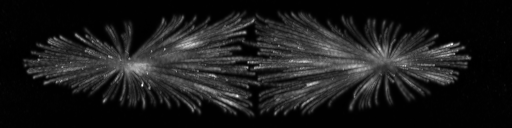
\includegraphics[width=\textwidth]{figures/MIPs/mip_DeconvOptim.png}
                \caption{\texttt{DeconvOptim.jl} . $\text{NCC}= 0.86$.}
            \end{subfigure}
            \begin{subfigure}{.3\textwidth}
                \centering
                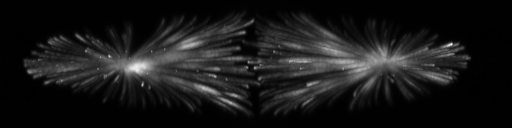
\includegraphics[width=\textwidth]{figures/MIPs/mip_DeconvOptim_RL.png}
                \caption{Julia Richardson-Lucy. $\text{NCC}= 0.74$.}
            \end{subfigure}
            \begin{subfigure}{.3\textwidth}
                \centering
                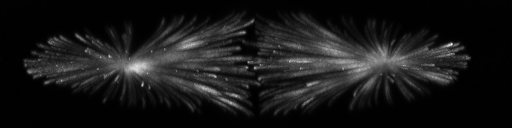
\includegraphics[width=\textwidth]{figures/MIPs/mip_DeconvolutionLab2.png}
                \caption{\texttt{Deconvolution Lab2}. $\text{NCC}= 0.76$.}
            \end{subfigure}
            \begin{subfigure}{.3\textwidth}
                \centering
                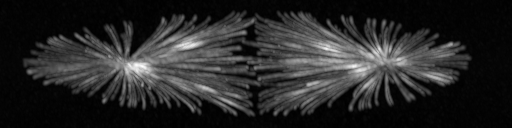
\includegraphics[width=\textwidth]{figures/MIPs/mip_ThreeDeconv.png}
                \caption{\texttt{ThreeDeconv.jl}. $\text{NCC}= 0.85$.}
            \end{subfigure}
            \begin{subfigure}{.3\textwidth}
                \centering
                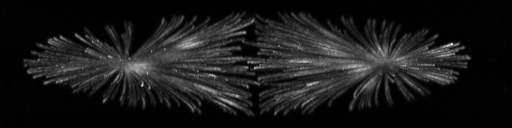
\includegraphics[width=\textwidth]{figures/MIPs/mip_GenericDeconv.png}
                \caption{\texttt{GenericDeconv}. $\text{NCC}= 0.86$.}
            \end{subfigure}
            \begin{subfigure}{.3\textwidth}
                \centering
                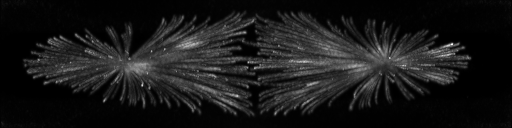
\includegraphics[width=\textwidth]{figures/MIPs/mip_Huygens.png}
                \caption{\texttt{Huygens}$\text{NCC}= 0.86$.}
            \end{subfigure}
            \begin{subfigure}{.3\textwidth}
                \centering
                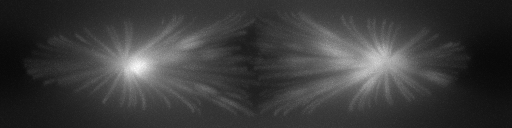
\includegraphics[width=\textwidth]{figures/MIPs/mip_raw.png}
                \caption{Measured image. $\text{NCC}= 0.41$.}
            \end{subfigure}
            \begin{subfigure}{.3\textwidth}
                \centering
                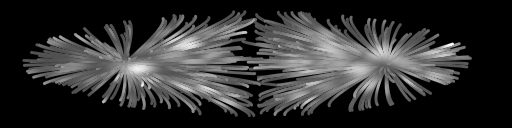
\includegraphics[width=\textwidth]{figures/MIPs/mip_ground_truth.png}
                \caption{Ground truth. $\text{NCC}= 1.0$}
            \end{subfigure}
            \caption{Maximum intensity projections along one dimensions of some of the deconvolution results.}
            \label{img:results}
        \end{figure} 

\section{Summary}
    In conclusion, \verb|DeconvOptim.jl| is a very performant, flexible deconvolution software to deconvolve multi-dimensional datasets.
    Its focus has been from the beginning to be fast and the source code should be automatic differentiated by the available
    packages in Julia. Usually we would expect that AD decreases performances but still our software is faster than
    many other packages which have been written with hand-optimized gradients.
    Furthermore, our toolbox is not restricted in dimensionality and has mechanism to prevent wrap-around artifacts which
    occur with FFT based convolutions.
    Julia's metaprogramming capabilities together with \verb|Tullio.jl| allow to generate regularizers which have high performance
    and are easy to adapt.
    In future, we want to support more regularizers on GPUs since they can not be handled efficiently with the current \verb|Tullio.jl| solution.
    Also we plan to extend the package to deconvolution of spatially varying kernels which are of importance in optical systems
    with large field of view or poor manufacturing quality.

\section{Acknowledgement}
    This work was partially funded by the Honours Programme of the Friedrich Schiller 
    University of Jena\footnote{\url{https://www.uni-jena.de/en/honours_programme}}.
    We want to thank Michael Abbott because he had the
    initial idea for the metaprogramming regularizers based on \verb|Tullio.jl|. 
    Additionally, we want to thank Scientific Volume Imaging for providing a trial license for Huygens and especially Mark Koenis for advising
    us how to adjust the settings to get optimal performance. 
\newpage
% **************GENERATED FILE, DO NOT EDIT**************

\bibliographystyle{juliacon}
\bibliography{ref.bib}


\end{document}
